\documentclass[11pt,a4paper]{article}

\usepackage{graphicx}
\usepackage{booktabs}
\usepackage{hyperref}
\usepackage{caption}
\usepackage{amsmath}
\usepackage{geometry}
\usepackage{enumitem}
\usepackage{xcolor}

\geometry{margin=2.5cm}
\graphicspath{{../Visualizations/}{../current_latest_paper/}}

\begin{document}

\section{Overview}

This document summarises the three analytical components contributed by Member~4 (Kusal Pabasara) to the research project. The work addresses three areas identified in the project proposal:
\begin{enumerate}[noitemsep]
  \item \textbf{Sensitivity Analysis} --- robustness of SHAP feature rankings across underemployment definitions
  \item \textbf{Gender Disaggregation} --- gender-specific driver structures and statistical testing
  \item \textbf{District-Level Analysis} --- spatial heterogeneity in underemployment patterns
\end{enumerate}

\section{Sensitivity Analysis: Hours-Based vs Qualification-Based Definitions}

\subsection{Methodology}
Parallel XGBoost-SHAP models were fitted using the same 7-predictor feature set on both the hours-based underemployment rate (DCS LFS, 2015--2024) and the qualification-based mismatch rate (computed from LFS micro-data, 2015--2023). Spearman rank correlation ($\rho$) was computed between the two SHAP importance rankings overall and by sub-period.

\subsection{Results}

\begin{table}[ht]
\caption{SHAP Feature Importance: Hours-Based vs Qualification-Based}
\label{tab:shap_sensitivity}
\setlength{\tabcolsep}{3pt}
\footnotesize
\begin{tabular}{lrrrrc}
\toprule
\textbf{Feature} & \textbf{Hours \%} & \textbf{Rank} & \textbf{Qual \%} & \textbf{Rank} & \textbf{$|\Delta|$}\\
\midrule
Exchange Rate & 34.0 & 1 & 75.8 & 1 & 0\\
GDP Growth & 21.3 & 2 & 8.5 & 2 & 0\\
Youth LFPR & 17.5 & 3 & 7.4 & 3 & 0\\
Agri. Output & 14.8 & 4 & 1.1 & 5 & 1\\
Informal Emp. & 10.0 & 5 & 0.6 & 6 & 1\\
Inflation$\dagger$ & 1.5 & 6 & 6.4 & 4 & 2\\
Remittances & 0.8 & 7 & 0.1 & 7 & 0\\
\midrule
\multicolumn{6}{l}{\scriptsize Spearman $\rho = 0.893$ ($p = 0.007$). $\dagger$Rank shift $\geq 2$.}\\
\bottomrule
\end{tabular}
\end{table}

The overall Spearman $\rho = 0.893$ ($p = 0.007$) confirms strong rank agreement, substantially exceeding the pre-registered threshold of $\rho > 0.6$. Exchange Rate, GDP Growth, and Youth LFPR retain the top three positions in both models. The main divergence is Inflation, which shifts from rank~6 (hours-based) to rank~4 (qualification-based).

\begin{table}[ht]
\caption{Sub-Period Definition Agreement (Spearman $\rho$)}
\label{tab:spearman_subperiod}
\footnotesize
\begin{tabular}{lccc}
\toprule
\textbf{Period} & \textbf{n} & \textbf{$\rho$} & \textbf{$p$}\\
\midrule
Pre-crisis (2015--2019) & 5 & 0.429 & 0.337\\
Crisis (2020--2022) & 3 & 0.786 & 0.036\\
Post-crisis (2023--2024) & 2 & -- & -- \\
\midrule
Overall & 10 & 0.893 & 0.007\\
\bottomrule
\end{tabular}
\end{table}

The qualification-based series shows a structural upward trend of $+0.87$ pp/year (64.2\% in 2015 to 70.9\% in 2023), indicating that occupational mismatch is worsening independently of the business cycle.

\begin{figure}[ht]
  \centering
  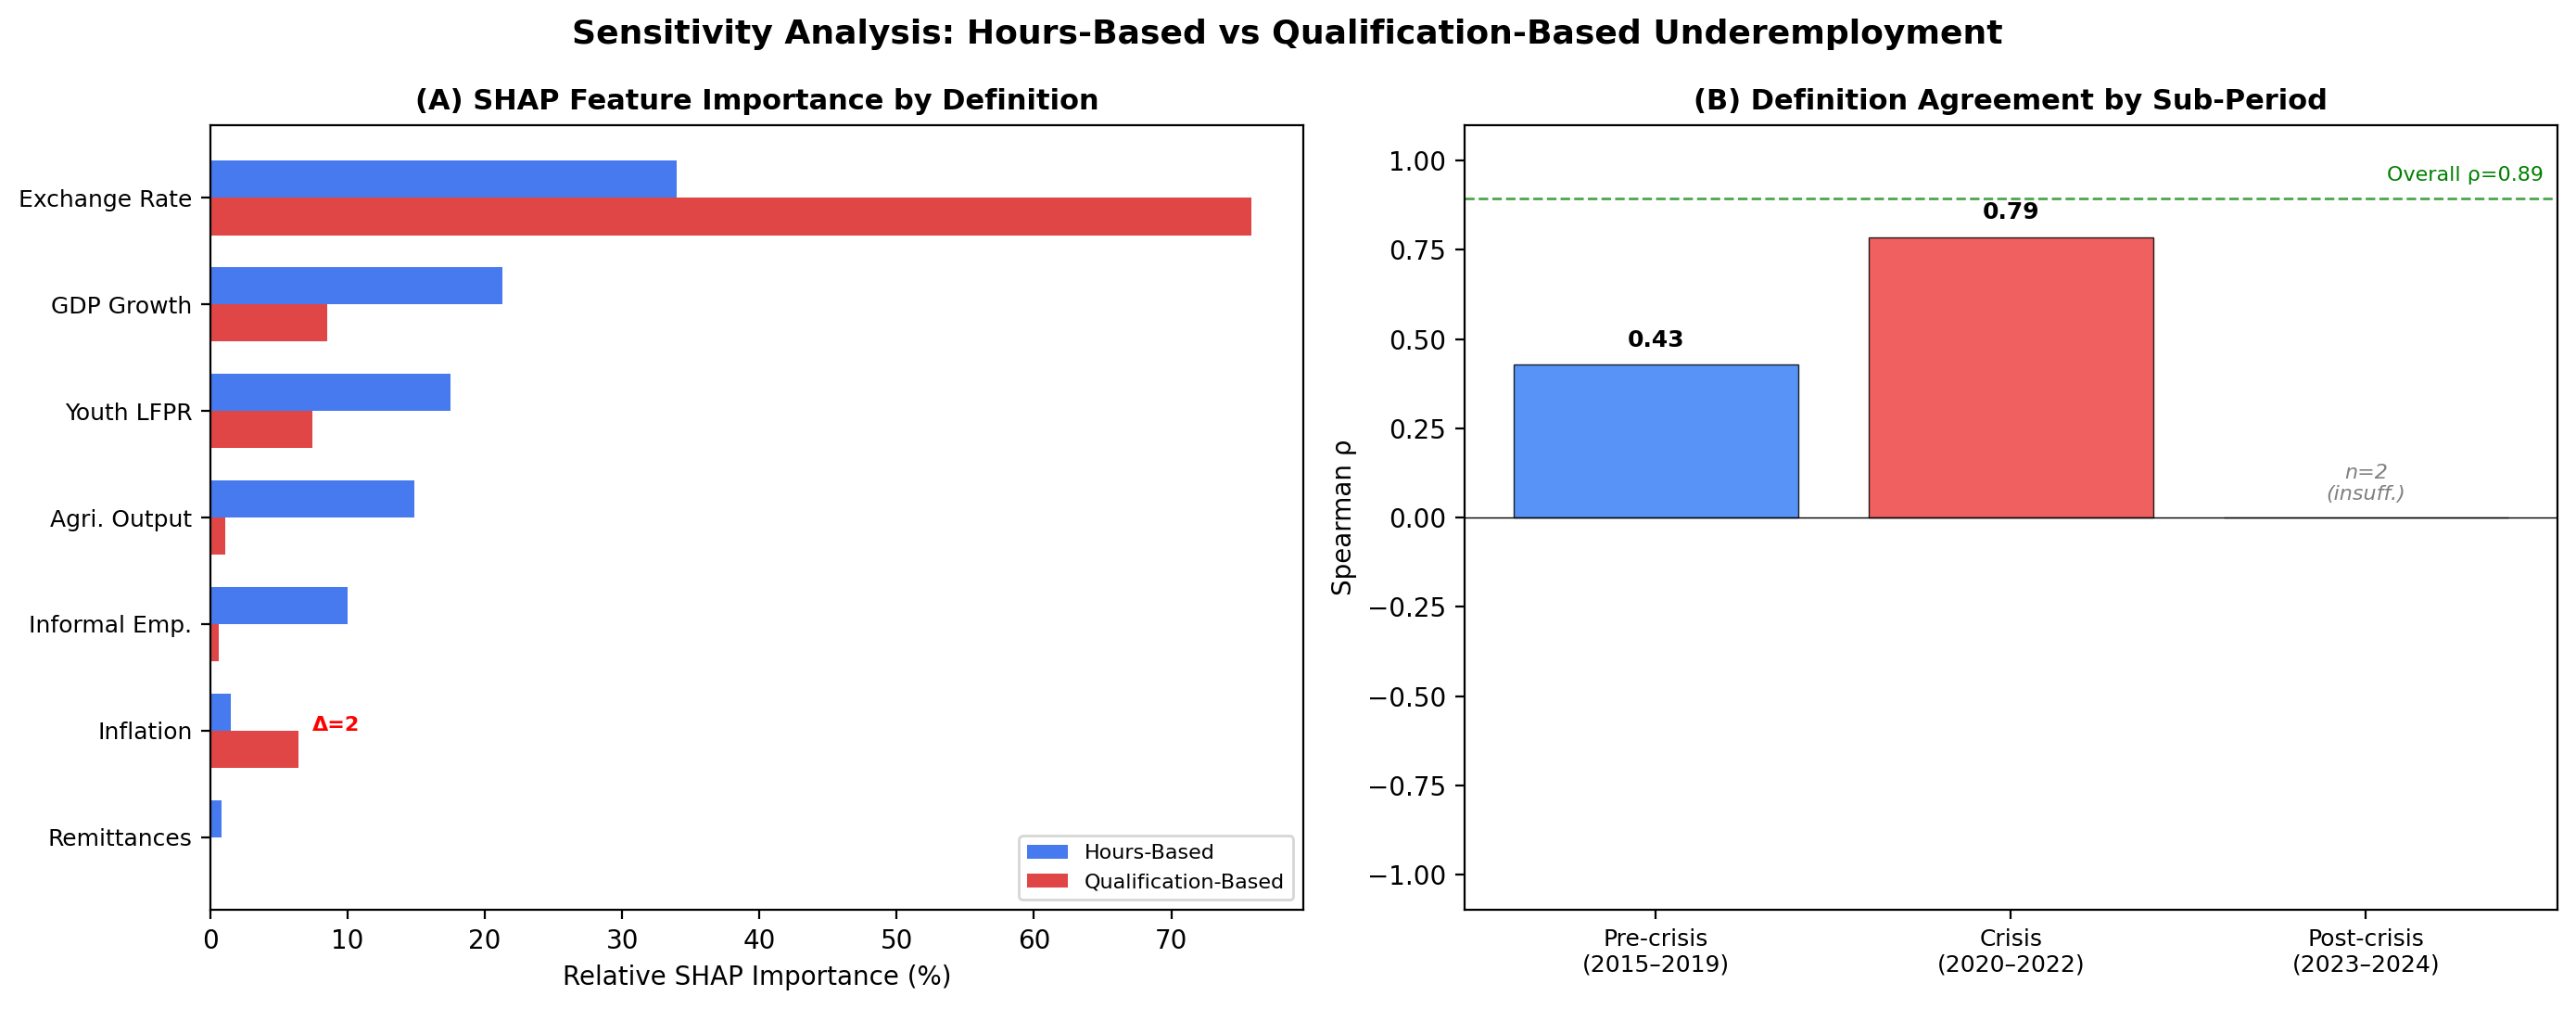
\includegraphics[width=0.85\textwidth]{sensitivity_shap_comparison.png}
  \caption{SHAP comparison: Hours-based (left) vs Qualification-based (right) models.}
  \label{fig:shap_comp}
\end{figure}

\begin{figure}[ht]
  \centering
  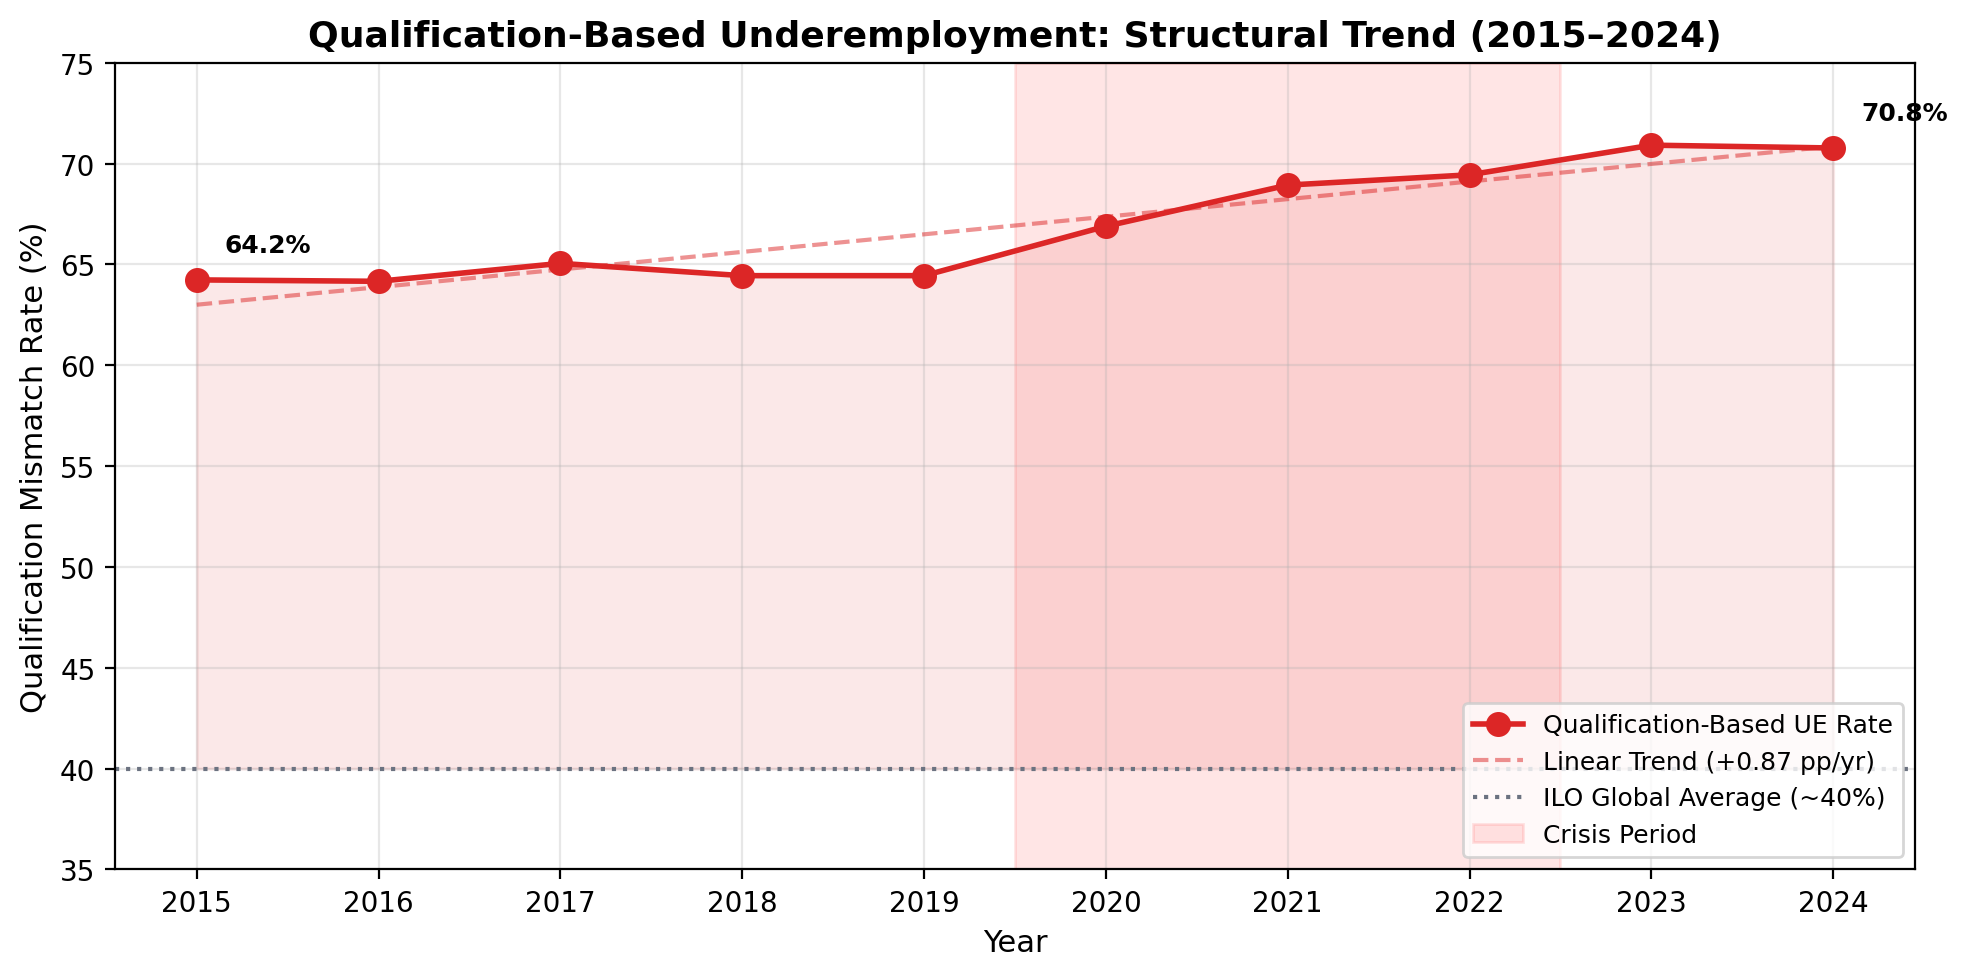
\includegraphics[width=0.85\textwidth]{sensitivity_qual_trend.png}
  \caption{Qualification-based underemployment trend (2015--2023) with OLS trend line and 95\% CI. Structural rise of $+0.87$ pp/year.}
  \label{fig:qual_trend}
\end{figure}

\section{Gender-Disaggregated Analysis}

\subsection{Methodology}
Gender-specific XGBoost-SHAP models were trained on female and male underemployment series from the DCS authoritative gender file (2015--2024). Statistical tests include Wilcoxon signed-rank (persistent gap), bootstrap confidence intervals (crisis-period gap), and Zivot-Andrews Model~C (structural break detection). The qualification-based gender gap was computed from LFS micro-data.

\subsection{Results}

\begin{table}[ht]
\caption{Gender-Disaggregated SHAP Feature Rankings}
\label{tab:gender_shap}
\setlength{\tabcolsep}{3pt}
\footnotesize
\begin{tabular}{lrrrrrr}
\toprule
\textbf{Feature} & \textbf{Agg \%} & \textbf{Rank} & \textbf{Female \%} & \textbf{Rank} & \textbf{Male \%} & \textbf{Rank}\\
\midrule
Exchange Rate & 49.4 & 1 & 41.4 & 1 & 48.5 & 1\\
Inflation & 17.2 & 2 & 33.3 & 2 & 16.8 & 3\\
GDP Growth & 10.6 & 3 & 4.2 & 5 & 20.4 & 2\\
Agri. Output & 8.1 & 4 & 0.0 & 7 & 5.5 & 5\\
Youth LFPR & 6.9 & 5 & 13.5 & 3 & 1.5 & 6\\
Remittances & 4.0 & 6 & 3.0 & 6 & 1.2 & 7\\
Informal Emp. & 3.8 & 7 & 4.6 & 4 & 6.1 & 4\\
\midrule
\multicolumn{7}{l}{\scriptsize Female--Male rank $\rho = 0.571$ ($p = 0.180$)}\\
\bottomrule
\end{tabular}
\end{table}

Key finding: \textbf{Inflation} is the second-ranked female driver (33.3\%) but third for males (16.8\%), while \textbf{GDP Growth} is second for males (20.4\%) but fifth for females (4.2\%). This indicates female underemployment is more price-sensitive and male underemployment is more demand-sensitive.

\begin{table}[ht]
\caption{Statistical Tests on the Gender Gap in Underemployment}
\label{tab:gender_gap_tests}
\footnotesize
\begin{tabular}{llrl}
\toprule
\textbf{Test} & \textbf{Statistic} & \textbf{$p$} & \textbf{Result}\\
\midrule
Mean gap (F$-$M) & 1.26~pp & -- & Persistent female excess\\
Shapiro-Wilk (gap) & $W=0.919$ & 0.351 & Normal\\
Wilcoxon signed-rank & $W=55.0$ & 0.0010 & Significant\\
Bootstrap CI (crisis) & [1.00, 1.20] & -- & Gap $>$ 0 at 95\%\\
ZA break (gap) & $t=-2.22$ & -- & Break: 2018 (--)\\
\bottomrule
\end{tabular}
\end{table}

The qualification-based gender gap widens dramatically from 0.97~pp (2015) to 4.42~pp (2021), indicating that the crisis disproportionately worsened female qualification mismatch.

\begin{figure}[ht]
  \centering
  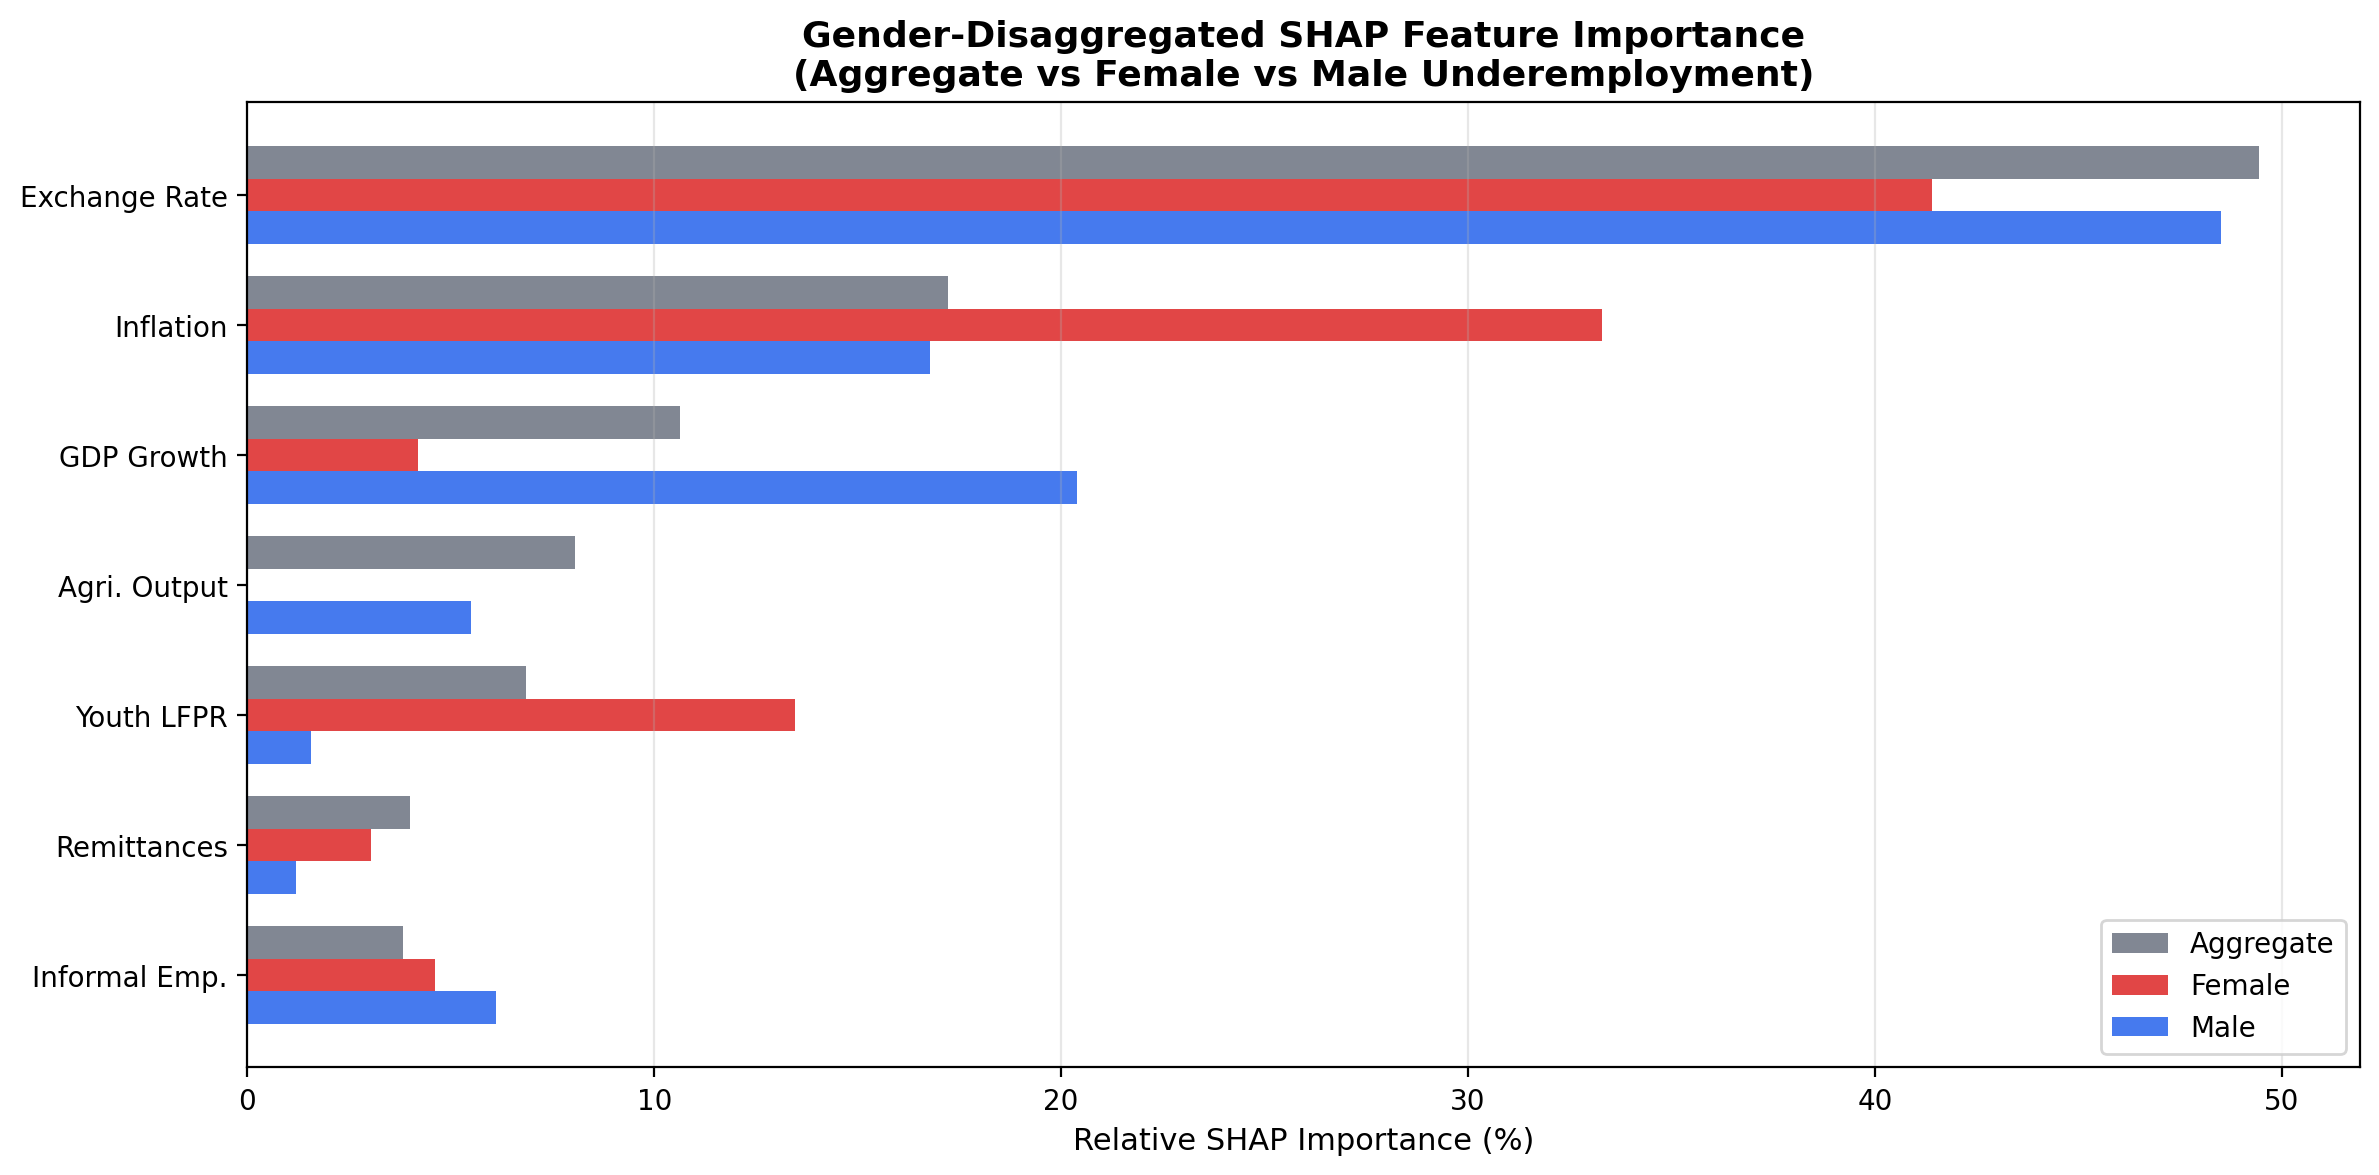
\includegraphics[width=0.85\textwidth]{gender_shap_comparison.png}
  \caption{SHAP feature importance: Aggregate vs Female vs Male models.}
  \label{fig:gender_shap}
\end{figure}

\begin{figure}[ht]
  \centering
  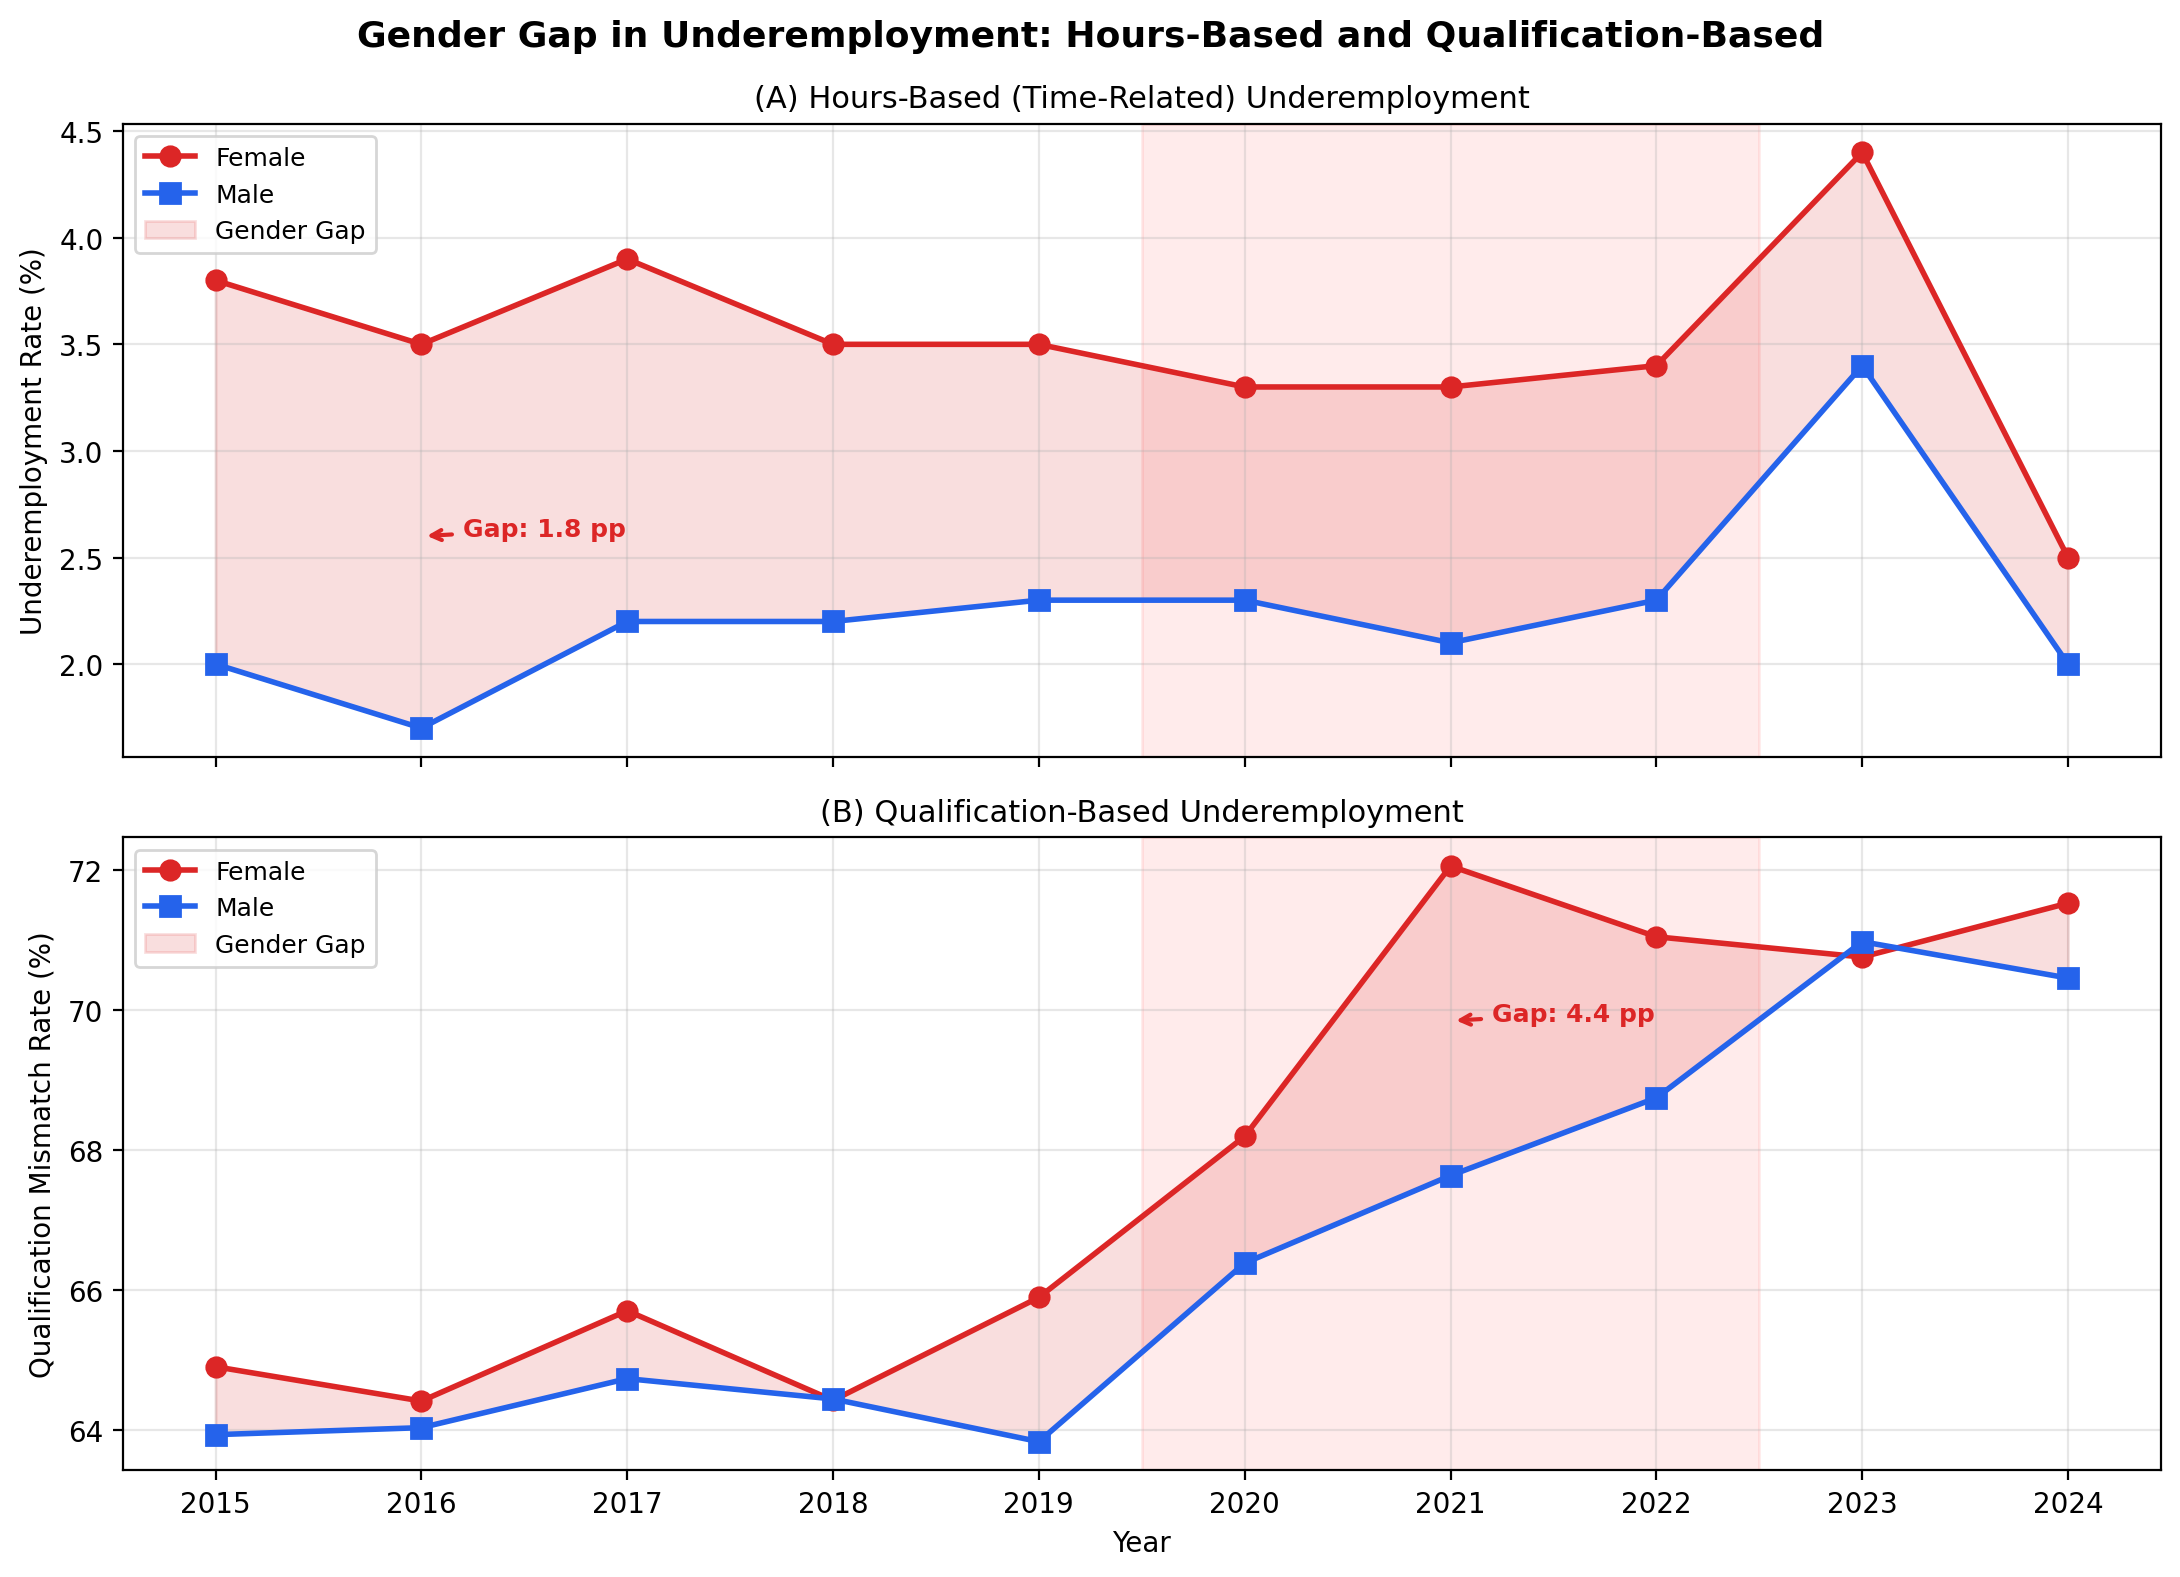
\includegraphics[width=0.85\textwidth]{gender_gap_extended.png}
  \caption{Gender gap trends: hours-based (DCS) and qualification-based mismatch. The qualification gap widens from 0.97~pp to 4.42~pp during 2015--2021.}
  \label{fig:gender_gap}
\end{figure}

\begin{figure}[ht]
  \centering
  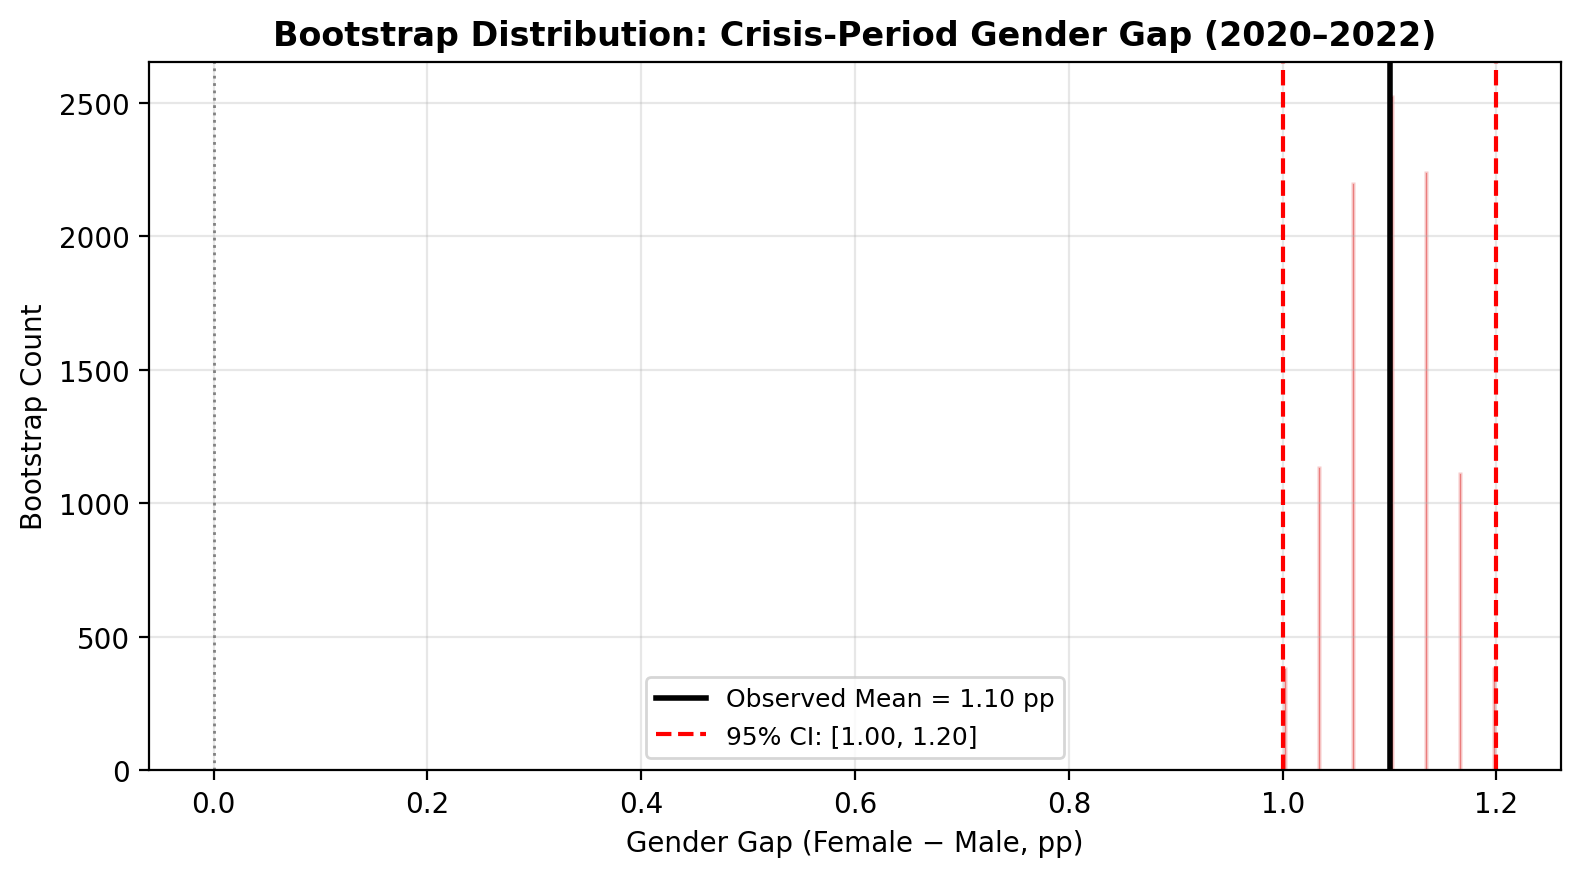
\includegraphics[width=0.85\textwidth]{gender_gap_statistical.png}
  \caption{Statistical visualisation: gap distribution, trend, and Wilcoxon results.}
  \label{fig:gender_stat}
\end{figure}

\section{District-Level Analysis}

\subsection{Methodology}
District-level data from DCS LFS Table~6.4 (25 districts, 2013--2022) was used to construct underemployment heatmaps, cross-sectional regressions of informal employment on underemployment, and priority district trajectory profiles.

\subsection{Results}

\begin{table}[ht]
\caption{District-Level Informal Employment vs Underemployment Regression}
\label{tab:district_regression}
\footnotesize
\begin{tabular}{lcccc}
\toprule
\textbf{Year} & \textbf{$n$} & \textbf{Slope} & \textbf{$R^2$} & \textbf{$p$}\\
\midrule
2019 & 25 & 0.0279 & 0.038 & 0.3508\\
2022 & 25 & 0.0204 & 0.059 & 0.2414\\
\bottomrule
\end{tabular}
\end{table}

Informality alone does not explain district-level underemployment variation ($R^2 < 0.06$, both years $p > 0.24$). Spatial heterogeneity is substantial: Colombo and Gampaha maintain below-average rates while Hambantota, Jaffna, and Mullaitivu are persistent hotspots.

\begin{figure}[ht]
  \centering
  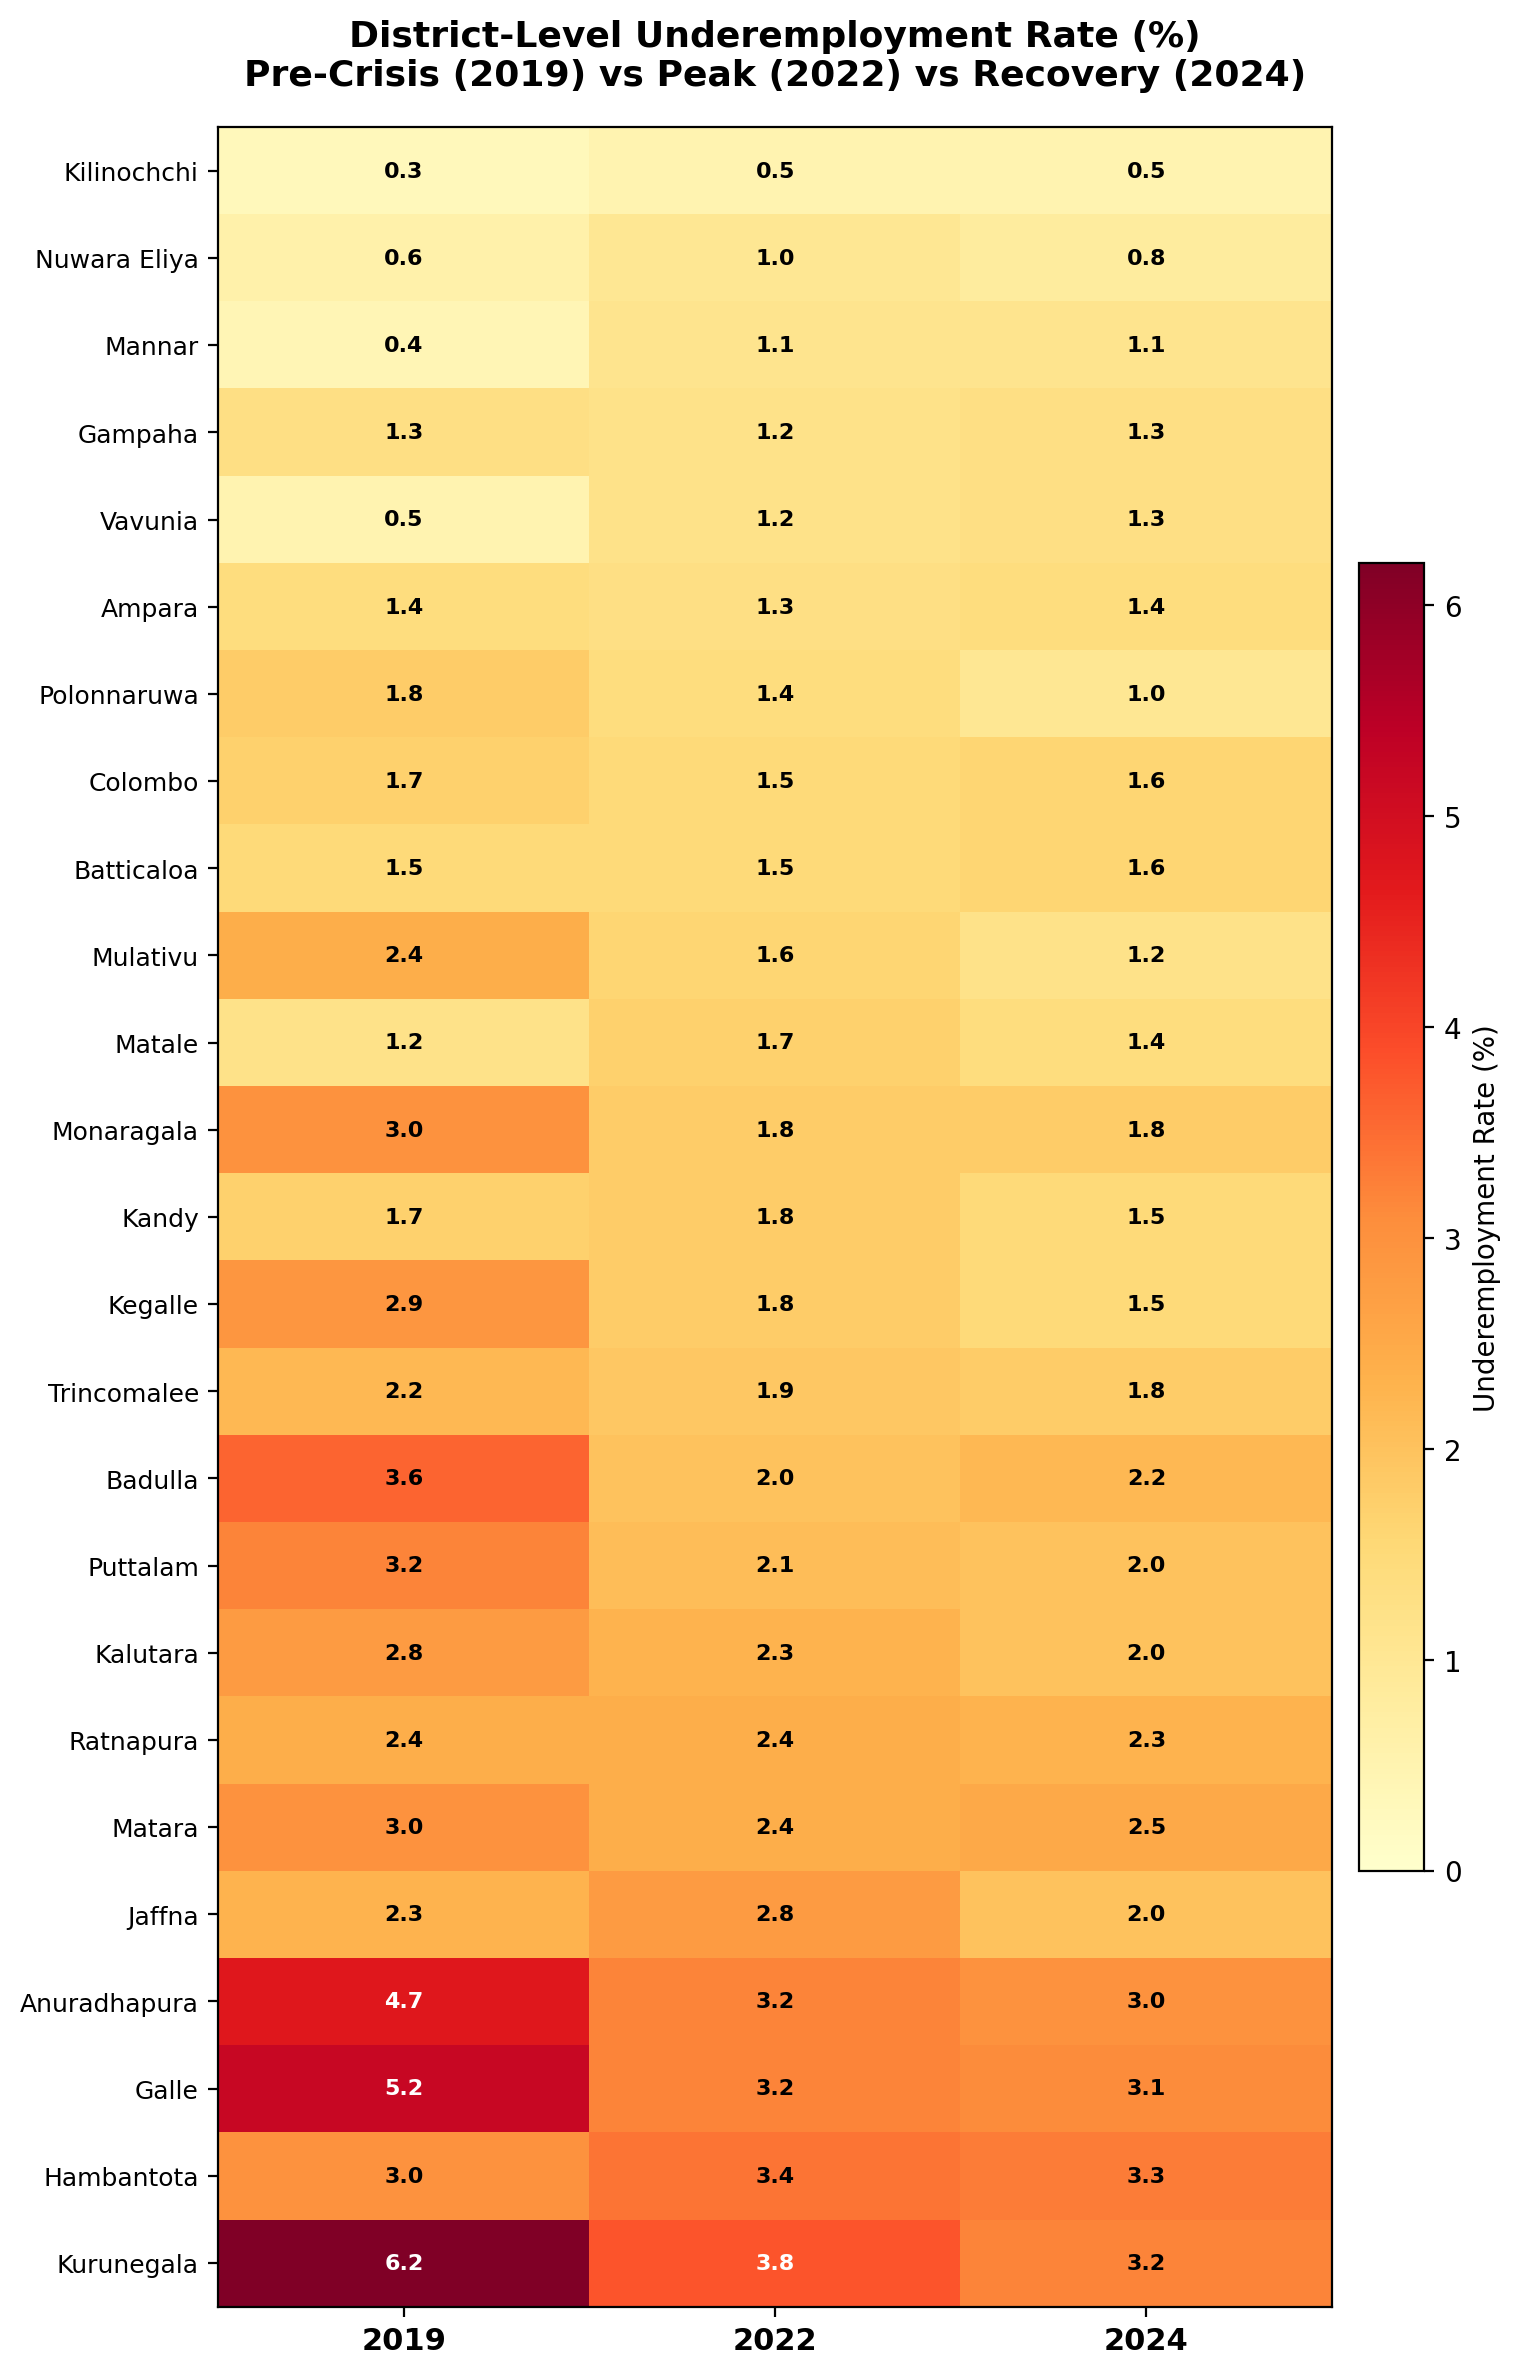
\includegraphics[width=0.85\textwidth]{district_heatmap.png}
  \caption{District-level underemployment heatmap (25 districts, 2019/2021/2022). Darker cells indicate higher underemployment.}
  \label{fig:district_heat}
\end{figure}

\begin{figure}[ht]
  \centering
  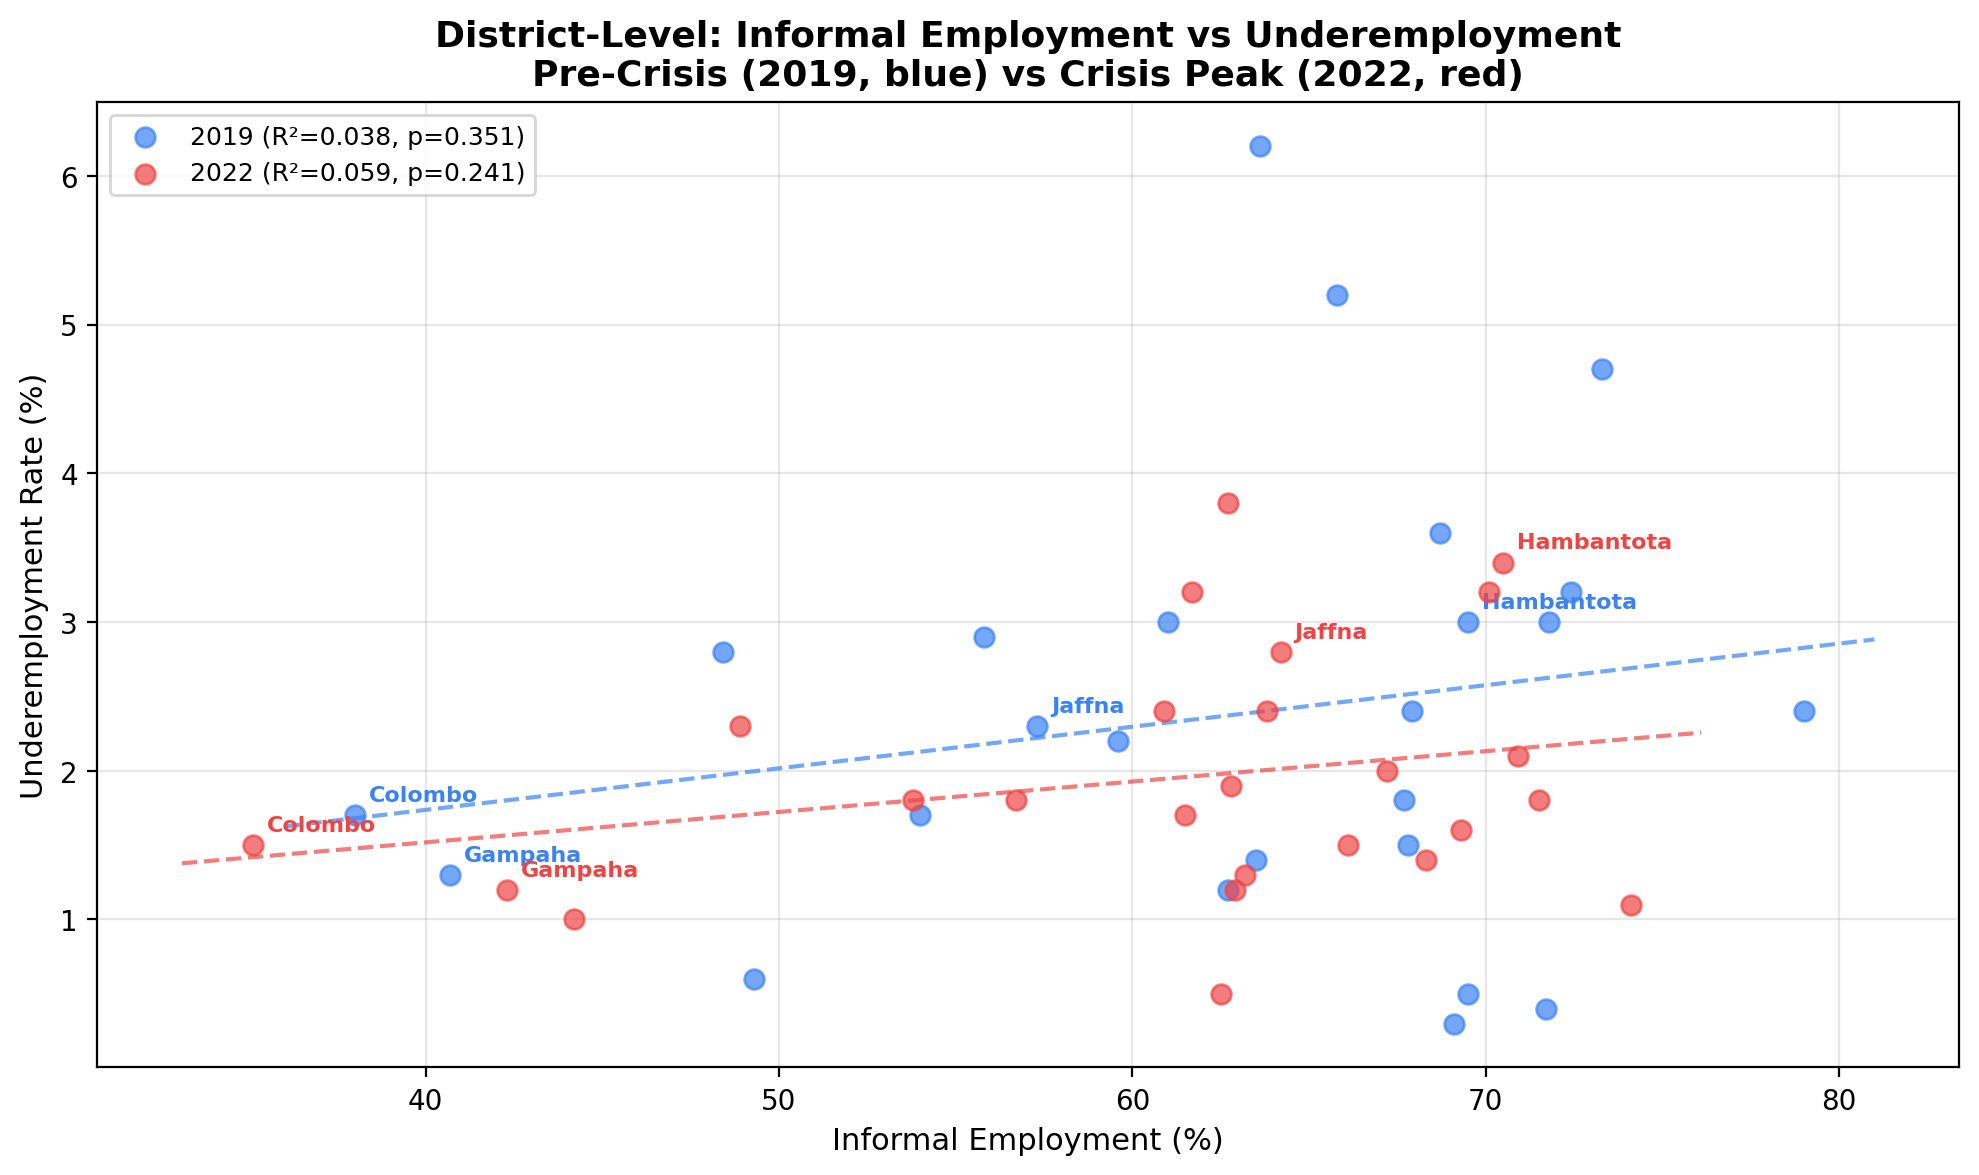
\includegraphics[width=0.85\textwidth]{district_informal_regression.png}
  \caption{Informal employment vs underemployment cross-sectional regression (2019 pre-crisis and 2022 crisis).}
  \label{fig:district_reg}
\end{figure}

\begin{figure}[ht]
  \centering
  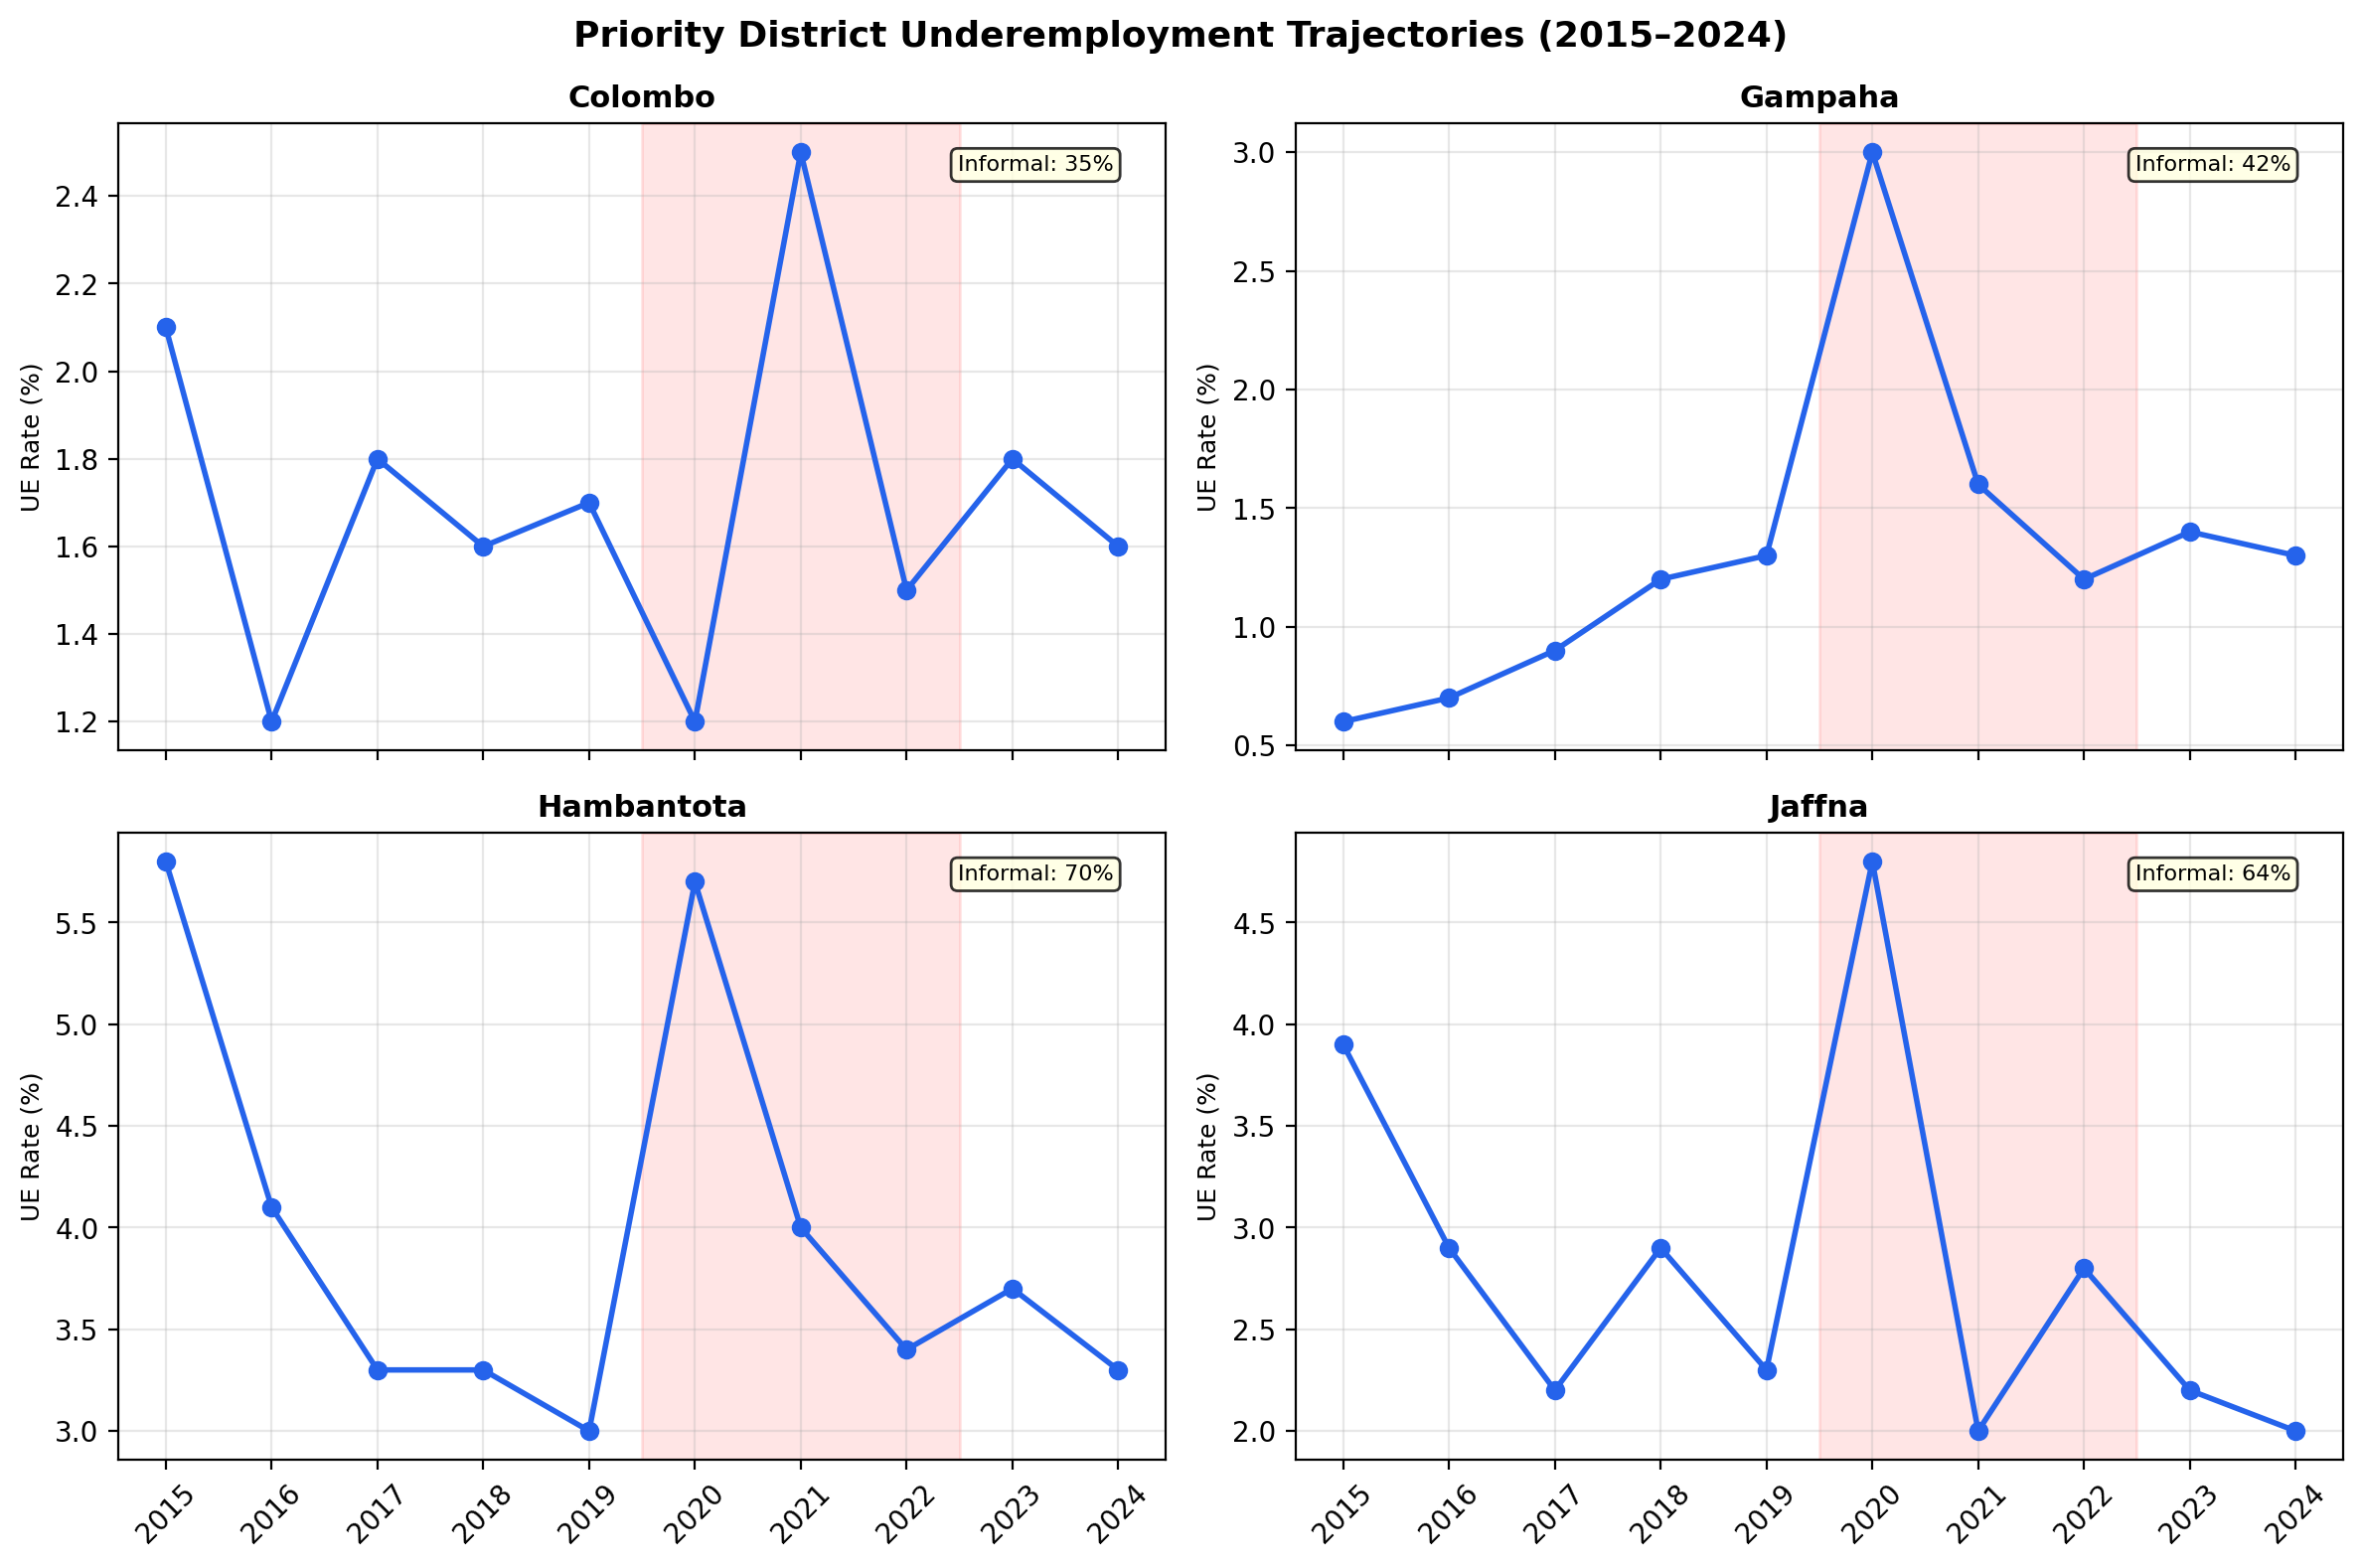
\includegraphics[width=0.85\textwidth]{district_profiles.png}
  \caption{Priority district trajectory profiles: Colombo, Gampaha, Hambantota, Jaffna.}
  \label{fig:district_prof}
\end{figure}

\section{Summary of Key Findings}

\begin{enumerate}[noitemsep]
  \item \textbf{Sensitivity}: SHAP rankings are strongly robust to definition choice ($\rho = 0.893$, $p = 0.007$); agreement strengthens during crisis periods.
  \item \textbf{Gender}: Female underemployment is inflation-driven; male is GDP-driven. The persistent female excess ($p = 0.001$) and widening qualification gap (0.97 $\to$ 4.42~pp) are novel findings for Sri Lanka.
  \item \textbf{District}: Substantial spatial heterogeneity exists that informality alone cannot explain; Northern and Southern districts are persistent hotspots requiring targeted policy.
\end{enumerate}

\section{Scripts and Outputs}

\begin{itemize}[noitemsep]
  \item \texttt{sensitivity\_analysis.py} $\to$ 2 figures, 2 LaTeX tables
  \item \texttt{gender\_analysis.py} $\to$ 3 figures, 2 LaTeX tables
  \item \texttt{district\_analysis.py} $\to$ 3 figures, 1 LaTeX table
\end{itemize}

All scripts are located in the repository root. Figures are saved to \texttt{Visualizations/} and LaTeX tables to \texttt{output/tables/}.

\end{document}
